\subsection{Adaptive Cruise Control in literature}

Adaptive cruise control (ACC) is an enhancement of the conventional cruise control which is currently standardised in most modern commercialised vehicles. The purpose of a classical cruise control is to maintain longitudinal vehicle velocity by tracking the velocity as requested by the driver. In ACC, there is an additional tracking of the velocity of the vehicle ahead and adapting to it, by accelerating or braking the vehicle independently of the driver. Typically, an external sensor such as a radar is used to detect the vehicle ahead and measure relative velocity between the vehicles \cite{Elsevier}.
ACC systems consist of two subsystems: a vehicle dependent part and a vehicle independent part. The former calculates a required acceleration/deceleration profile for the vehicle. The controller part forms the dependent part which tracks the profile by actuating the throttle and brake system \cite{Moon}. A schematic of the ACC system is shown in Fig. \ref{fig:Schematic_ACC}. 

\begin{figure}[h]
\centering
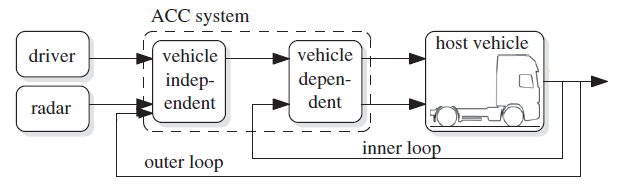
\includegraphics[width=0.45\textwidth]{img/ACC_schematic.png}\\
\caption{Schematic of ACC system \cite{Elsevier}}
\label{fig:Schematic_ACC}
\end{figure}
% Revisit schematic to also include the variables present in the figure

The main control objective is to follow the vehicle ahead. However, there are other aspects also considered such as comfort, fuel economy and safety \cite{Elsevier}. It should be noted that ACC is more of a comfort system than a safety system as the deceleration is limited to 3 $m/s^2$. Also, function of stop-and-go system can be integrated with ACC in order to allow the vehicle to stop behind vehicles at traffic signals or other conditions and continue again when the vehicle ahead begins to move \cite{ACC_SG}.  Also, driver mental workload was reduced with the implementation of ACC. Since ACC takes control from the driver, it should resemble the driver’s behaviour to a certain extent. Furthermore, constraints from subjective specific desirable behaviour should also be considered. Because of the need for constraints, classical controllers such as PID controller are insufficient. With LQR controller, it was found that the response of the system was slower compared with Model Predictive Controller (MPC) \cite{Takahama}. There are 2 approaches to design controllers for linear systems with constraints: anti-windup control and MPC. Former one demonstrates adequate performance on Single-Input Single-Output (SISO) situations, whereas MPC has outperformed in the field of complex constrained multi-variable (Multi-Input Multi-Output or MIMO) control problems. Other main advantages of MPC here would be the on-line optimisation of the system, stability and feasibility guarantee with closed loop MPC, and implementation in a receding horizon manner, where the optimization problem is solved in every time step. This enables the controller to adapt to actual working conditions, i.e. traffic situations, and, as such, the controller is situation dependent. The advantage of MPC for ACC is that high control performance can be obtained since constraints such as small feedback gain for LQR controller can be exclusively dealt with and the tuned weighing parameters can be intuitively and flexibly considered as a function of time considering various driving situations \cite{Takahama}.


% Also include the explanation of different sections of the paper.
\subsection{Model}

The host vehicle and target vehicle are modelled as in Fig. \ref{fig:ACC_example} with a relative distance.

\begin{figure}[h]
\centering
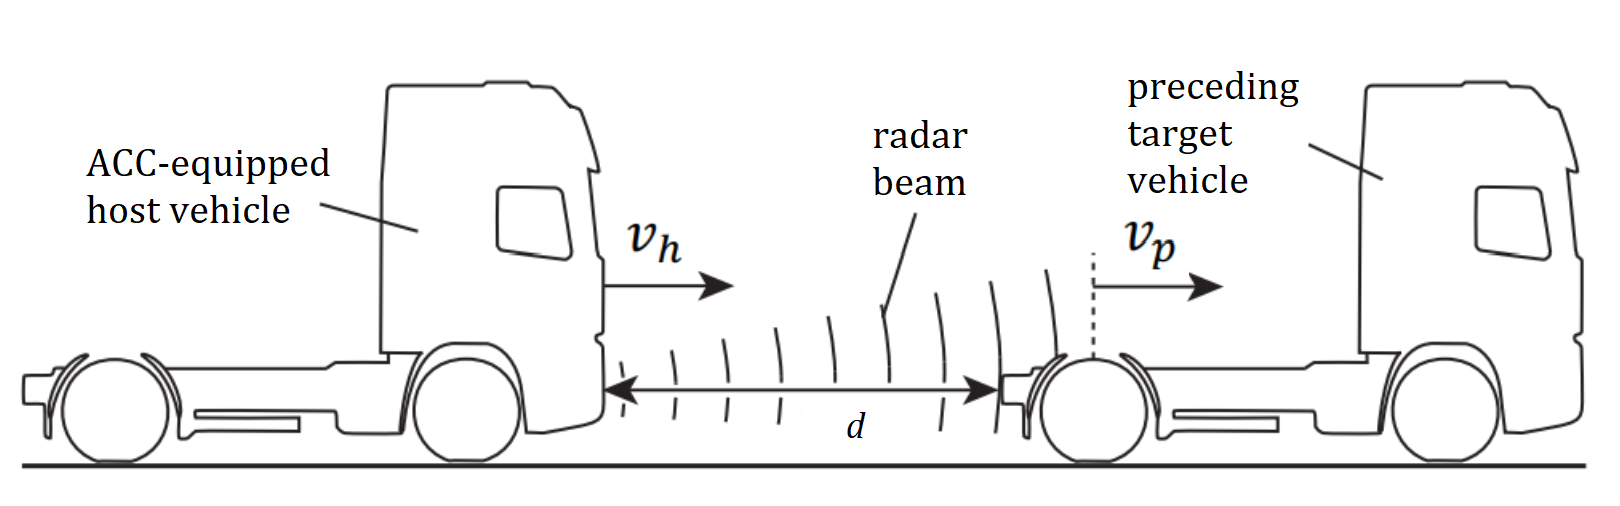
\includegraphics[width=0.45\textwidth]{img/trucks.png}\\
\caption{Example of ACC working principle. The host vehicle, driving with velocity $v_h$ and acceleration $a_h$, is equipped with ACC, which measures the preceding target vehicle, with velocity $v_t$. A radar measures the distance $x_r$ and the relative velocity $v_r=v_t-v_h$ between the vehicles. \cite{Elsevier}}
\label{fig:ACC_example}
\end{figure}

Since the purpose of ACC is to maintain a desired distance between host and target vehicle, a problem of the below considerations is taken,
\begin{itemize}
    \item The distance error $\delta d$, defined as difference between the inter-vehicle distance $d$ and desired distance $d_r$, where $\delta d = d - d_r$. This error should converge to zero.
    \item The velocity error $\delta v$, defined as the difference between the preceding target vehicle velocity $v_p$ and host velocity $v_h$. This error also should converge to zero.
    \item Acceleration of the host vehicle $\dot{v}_h$, which should also converge to zero.
\end{itemize}

A vehicle dynamics model is also considered to design MPC and analyse the controller performance. The longitudinal dynamics of the host vehicle is given as,
\[m\dot{v}_h = ma_f - r_{travel}\]
Here, m is the mass of the vehicle, $v_h$ the host vehicle velocity, $a_f$ is the traction force of the host vehicle converted to acceleration and $r_{travel}$ is the travel resistance consisting of several factors.
In general, the actuation dynamics can be described as an ordinary differential equation as below,
\begin{gather}
\begin{aligned}
\dot{x}_f &= f_{act}(x_f,u)\\
a_f &= h_{act}(x_f)
\end{aligned}
\end{gather}

where $x_f \in \mathbb{R} ^{n_f}$, $u \in \mathbb{R}$ are the states and the input to actuation system respectively. \textit{u} is the acceleration command calculated by the ACC controller. The output of the system is y = $a_f$. It is to be noted that since we are taking a simple model, we neglect the travel resistance $r_{travel}$ as it contains several factors which are vehicle specific. 

For the plant model of the ACC system, two primary state variables are taken, $\delta d$ and $\delta v$ as described earlier. The variable $d_r$ defined in $\delta d$ is given based on the constant time headway given as
\[d_r = T_{hw}v_h + d_0\]
where $T_{hw}$ is the constant time headway (the time needed for the host vehicle to reach the current position of the target vehicle) and $d_0$ is the stopping distance for safety margin. Here, we do not consider the stop-and-go function where the vehicle stops completely if the target vehicle stops. Hence we take $d_0$ as zero.

Now we define the state variable of the plant as,
\begin{align*}
    x = \begin{bmatrix}
    x_1 & x_2 & x_3^T
    \end{bmatrix}
\end{align*}
with $x_1 = \delta d$, $x_2 = \delta v$ and $x_3 = x_f$.\\
The state-space model can now be formulated as,
\begin{gather}
\begin{aligned}
\dot{x}_f &= A_f(t)x_f + B_f(t)u\\
a_f &= C_f x_f
\end{aligned}
\end{gather}

where the state $x_f \in \mathbb{R}$, i.e. $n_f=1$ and

\begin{equation}
A_f(t) =
\begin{cases}
& -\frac{1}{T_{eng}},\: \text{if}\: u(t) \geq a_{thr\_off}\\
& -\frac{1}{T_{brk}},\: \text{if}\: u(t) < a_{thr\_off}
\end{cases}
\end{equation}

\begin{equation}
B_f(t) =
\begin{cases}
& -\frac{K_{eng}(t)}{T_{eng}},\: \text{if}\: u(t) \geq a_{thr\_off}\\
& -\frac{K_{brk}(t)}{T_{brk}},\: \text{if}\: u(t) < a_{thr\_off}
\end{cases}
\end{equation}

\[
C_f = 1
    % \begin{bmatrix}
    % 1 & 0 & 0\\
    % 0 & 1 & 0\\
    % 0 & 0 & 1
    % \end{bmatrix}
\]

$T_{eng}$ and $T_{brk}$ are given respectively as the time constant of acceleration using engine and deceleration using brake, $a_{thr.off}$ is the acceleration generated when the throttle valve is closed, $K_{eng}(t)$ and $K_{brk}(t)$ are the steady-state gains dependent on time. In the system (1), the dynamics is separated into acceleration and deceleration side and simply modeled as first-order delay system. Therefore, the overall simplified linear state-space model with the three states can be written as,
\begin{gather}
\begin{aligned}
\dot{x} &= A(t)x + B(t)u\\
y &= Cx
\end{aligned}
\end{gather}

where $x \in \mathbb{R}^3$ and

\[
A(t)=
    \begin{bmatrix}
    0 & 1 & -T_{hw}\\
    0 & 0 & -1\\
    0 & 0 & A_f(t)
    \end{bmatrix},
    \quad
B(t)=
\begin{bmatrix}
0\\
0\\
B_f(t)
\end{bmatrix}
\]

This model will be used for our MPC problem. For a non-linear system, it is necessary to linearize the system around the equilibrium. However, since we have already considered a linear system, we directly discretize the system from continuous time to discrete time. In MATLAB, this is done using the \textit{c2d} command. By doing so, we get the below discretized model.
\begin{gather}
\begin{aligned}
    x_{t+1} &= \Pi(t) x_t + \Gamma(t) u_t\\
    y_t &= C_d x_t
\end{aligned}
\end{gather}

$\Pi(t) = (I+T_S A(t)),\, \Gamma(t)=T_S B(t)$ and $C_d=C$ where $T_S$ is the sampling time.

% from MATLAB we need to write the values and rewrite the above equation.
    

